\section{Описание}

Задача о принадлежности точки многоугольнику является фундаментальной темой в вычислительной геометрии. Существует много алгоритмов для решени данной задачи, такие как метод трассировки лучей, учёт числа оборотов, суммирование углов. Все эти алгоритмы работают без предварительной обработки фигуры. В данной работе мне пришлось работать с препроцессингом, использующим персистентную структуру данных (сбалансированное AVL-дерево). 

Допустим, что у нас есть фигуры, изображенные на рис. 1. 

\begin{figure}[h]
  \subfigure[][рис. 1]{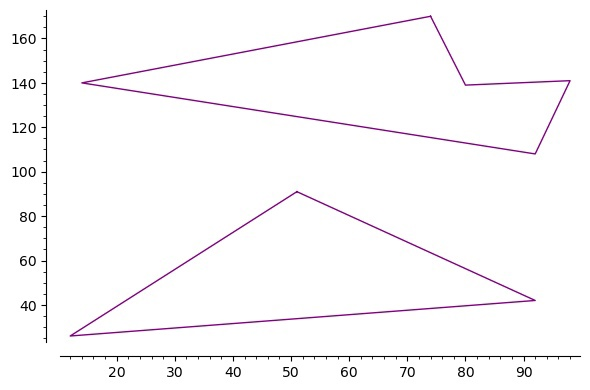
\includegraphics[scale=0.4]{../plots/1.jpg}}
  \subfigure[][рис. 2]{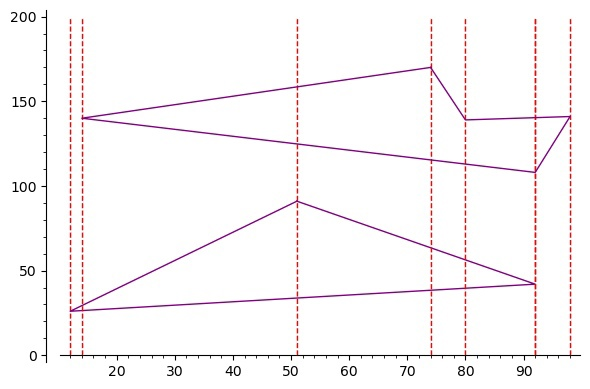
\includegraphics[scale=0.4]{../plots/2.jpg}}
\end{figure}

Тогда всю плоскость можно мысленно разбить на плиты (slabs в английской литературе), проведя через каждую точку вертикальную прямую (рис. 2). 

Если многоугольники без самопересечений, то мы можем гарантировать, что внутри каждой плиты отрезки, полученные разбиением ребер можно упорядочить (определить оператор отношения).
 
Вообще если брать произвольные отрезки, то упорядочить их невозможно, однако разбиение на плиты позволяет нам это сделать. Таким образом сложность поиска должна составить $O(log_2^2(n))$  

\begin{figure}[h]
  \subfigure[][рис. 3]{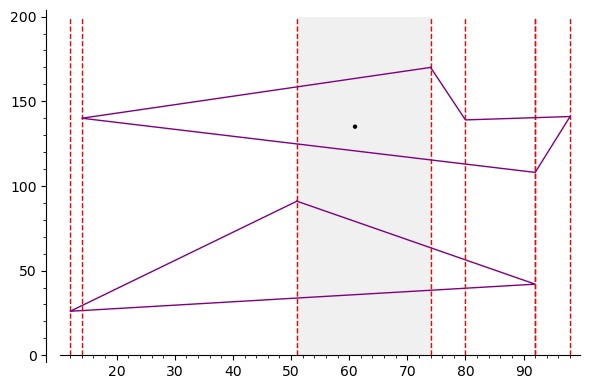
\includegraphics[scale=0.4]{../plots/3.jpg}}
  \subfigure[][рис. 4]{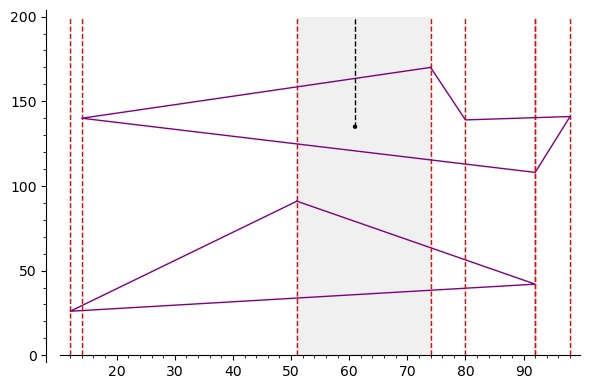
\includegraphics[scale=0.4]{../plots/4.jpg}}
\end{figure}

Подав точку на вход мы можем бинарным поиском найти нужную нам плиту (рис. 3) (для этих целей служит отсортированный массив x'ов), после чего в дереве искать место, между какими ребрами попала точка. Если в процессе препроцессинга хранить в дереве количество ребер выше (т.е. в правом поддереве), то можно за логарифмическую сложность узнать, сколько ребер находится над точкой и по методу трассировки лучей (рис. 4), выдать ответ о принадлежности точки многоугольнику. Номер многоугольника выбирается за счет хранения и запоминания в процессе поиска в дереве номера фигуры соответствующего пройденному ребру.

Сложность препроцессинга же $O(nlog(n))$, что можно будет заметить на тестах.

\newpage

\section{Исходный код}

Классы точки и ребра - простые библиотеки с множеством методов и конструкторов, позволяющие абстрактно использовать их в ходе всего курсового проекта. Так как в основном вся реализация простая, то я не буду включать их в листинг курсовой.

\begin{lstlisting}[language=c++]

#pragma once
#include <iostream>
#include <math.h>
#include <cfloat>
#include <fstream>

class Point {
	public:
		double x;
		double y;
		Point(double _x = 0.0, double _y = 0.0);
		Point operator+ (const Point&) const;
		Point operator- (const Point&) const;
		friend Point operator* (const double, const Point&);
		double operator[] (int);
		bool operator== (Point) const;
		bool operator< (Point) const;
		bool operator> (Point) const;
		bool operator!= (Point) const;
		int classify(Point, Point);
		double polarAngle(void);
		double length(void);
		double distance(Point&, Point&);
		friend std::ostream& operator<<(std::ostream&, const Point&);
};

enum {
	LEFT,
	RIGHT,
	BEYOND,
	BEHIND,
	BETWEEN,
	ORIGIN,
	DESTINATION
};

class Edge {
	public:
		Point org;
		Point dest;
		Edge(void);
		Edge(double p1_x, double p1_y, double p2_x, double p2_y);
		Edge(Point& _org, Point& _dest);
		Edge(Point& _org, Point&& _dest);
		Edge& rot(void);
		Edge& flip(void);
		Point point(double);
		int intersect(Edge&, double&);
		int intersect(Edge&&, double&);
		int cross(Edge&, double&);
		bool isVertical(void);
		double slope(void) const;
		double y(double) const;
		bool abovePoint(Point) const;
		bool underPoint(Point) const;
		bool crossPoint(Point) const;
		bool operator==(Edge) const;
		bool operator!=(Edge) const;
		double min_y() const;
		double max_y() const;
		friend std::ofstream& operator<<(std::ofstream&, const Edge&);
		friend std::ostream& operator<<(std::ostream&, const Edge&);
		friend std::ifstream& operator>>(std::ifstream&, Edge&);
};

enum {
	COLLINEAR,
	PARALLEL,
	SKEW,
	SKEW_CROSS,
	SKEW_NO_CROSS
};
\end{lstlisting}

Самый важный класс из курсового проекта - персистентное сбалансированное AVL-дерево. О методах подробнее в таблице:

\begin{longtable}{|p{7.5cm}|p{7.5cm}|}
\hline
\rowcolor{lightgray}
\multicolumn{2}{|c|} {persistent\_tree2.hpp}\\
\hline
PersistentTree::Insert (const K\&, const V\&, const double, const bool) & Вставка в персистентное дерево. Булевый флаг указывает, сохранять ли новую версию дерева или нет\\
\hline
PersistentTree::Remove (const K\&, const double, const bool) & Удаление из дерева по ключу с такой же функцией у булевого флага\\
\hline
PersistentTree::NotChange () & Копирование самой последней версии \\
\hline
PersistentTree::FindNumberAbove (const unsigned int, const Point\&, long*, long*) & Возвращает количество рёбер над точкой\\
\hline
PersistentTree::Print (...) & Вывод дерева в консоль\\
\hline
PersistentTree::operator<< (ofstream\&, PersistentTree\&) & Сохранение дерева в файл\\
\hline
PersistentTree::operator>> (ifstream\&, PersistentTree\&) & Загрузка дерева из файла\\
\hline
\end{longtable}

\begin{lstlisting}[language=c++]
#pragma once

#include <iostream>
#include <vector>
#include <memory>
#include <map>
#include <unordered_map>
#include <queue>
#include "utilitys.hpp"

using namespace std;

static unsigned long long index = 1;

template<class K, class V>
struct PersistentTree {

	struct node {

		using h_type = unsigned int;
		using nre_type = unsigned int;
		using idx_type = unsigned long long;
		using node_ptr = shared_ptr<node>;

		node_ptr l = nullptr;
		node_ptr r = nullptr;
		K key;
		V value;
		h_type h;
		nre_type nre;
		idx_type idx;

		node(const K& _k, const V& _v): key(_k), value(_v), h(1), nre(0) {
			idx=index; 
			index++;
		}
		node(const K& _k, const V& _v, const h_type& _h, const nre_type& _nre): key(_k), value(_v), h(_h), nre(_nre) {
			idx=index; 
			index++;
		}

		node_ptr RightRotate(node_ptr head) {
			node_ptr temp1 = make_shared<node>(head->l->key, head->l->value, head->l->h, 1 + head->l->nre + head->nre);
			node_ptr temp2 = make_shared<node>(head->key, head->value, head->h, head->nre);
			temp1->l = head->l->l;
			temp1->r = temp2;
			temp2->l = head->l->r;
			temp2->r = head->r;
			FixHeight(temp2);
			FixHeight(temp1);
			return temp1;
		}

		node_ptr LeftRotate(node_ptr head) {

			if (head->key == head->r->key)
				return head;

			node_ptr temp1 = make_shared<node>(head->r->key, head->r->value, head->r->h, head->r->nre);
			node_ptr temp2 = make_shared<node>(head->key, head->value, head->h, head->nre - 1 - head->r->nre);
			temp1->l = temp2;
			temp1->r = head->r->r;
			temp2->l = head->l;
			temp2->r = head->r->l;
			FixHeight(temp2);
			FixHeight(temp1);
			return temp1;
		}

		node_ptr Balancing(node_ptr head) {
			node_ptr temp = make_shared<node>(head->key, head->value, head->h, head->nre);
			temp->l = head->l;
			temp->r = head->r;
			FixHeight(temp);
			if (Balance(temp)==2) {
				if (Balance(temp->l)<0) {
					temp->l = LeftRotate(head->l);
				}
				return RightRotate(temp); 
			} else if (Balance(temp)==-2) {
				if (Balance(temp->r)>0) {
					temp->r = RightRotate(head->r);
				}
				return LeftRotate(temp);
			}
			return temp;
		}

		node_ptr Insert(const node_ptr parent, const K& key, const V& value, const double slab) {
			static unsigned int index = 1;
			if (parent) {
				node_ptr temp;
				if (key.y(slab) > parent->key.y(slab)) {
					temp = make_shared<node>(parent->key, parent->value, parent->h, parent->nre + 1);
					temp->l = parent->l;
					temp->r = Insert(parent->r, key, value, slab);
				} else {
					temp = make_shared<node>(parent->key, parent->value, parent->h, parent->nre);
					temp->r = parent->r;
					temp->l = Insert(parent->l, key, value, slab);
				}

				return Balancing(temp);
			}

			return make_shared<node>(key, value);
		}

		node_ptr MinRight(node_ptr head) {
			node_ptr temp = head;
			while (temp->l) {
				temp = temp->l;
			}
			return temp;
		}

		node_ptr RemoveMin(node_ptr head) {
			if (!head->l) {
				node_ptr temp = head->r;
				return temp;
			}
			node_ptr temp = make_shared<node>(head->key, head->value, head->h, head->nre);
			temp->r = head->r;
			temp->l = RemoveMin(head->l);
			return Balancing(temp);
		}

		node_ptr Remove(node_ptr parent, const K& key, const double slab) {
			if (!parent) 
				return nullptr;

			node_ptr temp;
			if (key == parent->key) {
				if (!parent->l and !parent->r) {
					return nullptr;
				}

				if (!parent->r) {
					return parent->l;
				}

				node_ptr min_right = MinRight(parent->r);
				temp = make_shared<node>(min_right->key, min_right->value, parent->h, parent->nre - 1);
				temp->l = parent->l;
				temp->r = RemoveMin(parent->r);
			} else if (key.y(slab) < parent->key.y(slab)) {
				temp = make_shared<node>(parent->key, parent->value, parent->h, parent->nre);
				temp->r = parent->r;
				temp->l = Remove(parent->l, key, slab);
			} else {
				temp = make_shared<node>(parent->key, parent->value, parent->h, parent->nre - 1);
				temp->l = parent->l;
				temp->r = Remove(parent->r, key, slab);
			}
			
			return Balancing(temp);
		}

		nre_type FindNumberAbove(const node_ptr head, const Point& p, bool *onEdge, long* left_ancestor, long* right_ancestor) {
			if (head) {
				if (p.y > head->key.y(p.x)) {
					*left_ancestor = static_cast<long>(head->value);
					return FindNumberAbove(head->r, p, onEdge, left_ancestor, right_ancestor);
				} else if (p.y == head->key.y(p.x)) {
					*left_ancestor = static_cast<long>(head->value);
					*right_ancestor = static_cast<long>(head->value);
					*onEdge = true;
					return 0;
				} else {
					*right_ancestor = static_cast<long>(head->value);
					return head->nre + 1 + FindNumberAbove(head->l, p, onEdge, left_ancestor, right_ancestor);
				}
			}

			return 0;
		}

		h_type Height(const node_ptr head) const {
			return head ? head->h : 0;
		}

		int Balance(const node_ptr head) const {
			return head ? Height(head->l)-Height(head->r) : 0;
		}

		void FixHeight(node_ptr head) {
			head->h = (Height(head->l)>Height(head->r) ? Height(head->l) : Height(head->r))+1;
		}

		void Print(const node_ptr head, unsigned int tab) const {
			if (head) {
				Print(head->r, tab + 1);
				for (unsigned int i = 0; i < tab; i++) std::cout << "\t";
				std::cout << "(" << head->key << ", " << head->value << ", " << head->h << ", " << head->nre << ", " << head->idx << ")\n";
				Print(head->l, tab + 1);
			}
		}

		friend std::ostream& operator<<(std::ostream& out, const node& p) {
			out << p.key << " " << p.value << " " << p.h << " " << p.nre << " " << p.idx;
			return out;
		}

		friend std::ofstream& operator<<(std::ofstream& out, const node& p) {
			out << p.key << " " << p.value << " " << p.h << " " << p.nre << " " << p.idx;
			return out;
		}

	};

	using node_ptr = shared_ptr<node>;

	unsigned int number_of_versions = 0;
	vector<node_ptr> trees;

	void Insert(const K& key, const V& value, const double slab, const bool flag = false) {
		if (!flag) {
			if (trees.empty()) {
				trees.push_back(nullptr);
				trees[0] = make_shared<node>(key, value);
			} else {
				trees.push_back(nullptr);
				trees[number_of_versions] = trees[number_of_versions]->Insert(trees[number_of_versions - 1], key, value, slab);
			}
			number_of_versions++;
		} else {
			if (trees.empty()) {
				trees.push_back(nullptr);
				trees[0] = make_shared<node>(key, value);
				number_of_versions++;
			} else {
				trees[number_of_versions - 1] = trees[number_of_versions - 1]->Insert(trees[number_of_versions - 1], key, value, slab);
			}
		}
	}

	void Remove(const K& key, const double slab, const bool flag = false) {
		if (!flag) {
			trees.push_back(nullptr);
			trees[number_of_versions] = trees[number_of_versions]->Remove(trees[number_of_versions - 1], key, slab);
			number_of_versions++;
		} else {
			trees[number_of_versions - 1] = trees[number_of_versions - 1]->Remove(trees[number_of_versions - 1], key, slab);
		}
	}

	void NotChange() {
		trees.push_back(nullptr);
		trees[number_of_versions] = trees[number_of_versions - 1];
		number_of_versions++;
	}

	unsigned int FindNumberAbove(const unsigned int version, const Point& p, long* left_ancestor, long* right_ancestor) {
		if (version >= trees.size()) {
			print("bad version: ", version);
			throw "There is no such version";
		}

		bool onEdge = false;
		unsigned int result = trees[version]->FindNumberAbove(trees[version], p, &onEdge, left_ancestor, right_ancestor);

		if (onEdge) 
			result = 1;

		return result; 
	}

	void Print(const unsigned int version) const {
		if (version >= trees.size()) {
			cout << "|--------------------------------------------------|" << endl;
			cout << "There is no such version of tree" << endl;
			cout << "|--------------------------------------------------|" << endl;
			return;
		}

		cout << "|--------------------------------------------------|" << endl;
		cout << "[" << version << "]" << endl;
		trees[version]->Print(trees[version], 0);
		cout << "|--------------------------------------------------|" << endl;
	}

	void Print() const {
		unsigned int v = 1;
		cout << number_of_versions << " versions in total:\n";
		for (node_ptr tree : trees) {
			cout << "|--------------------------------------------------|" << endl;
			cout << "[" << v << "]" << endl;
			tree->Print(tree, 0);
			cout << "|--------------------------------------------------|" << endl;
			v++;
		}
	}

	friend ofstream& operator<<(ofstream& out, PersistentTree& pt) {
		map<unsigned long long, node> visited;

		node_ptr curr;
		out << pt.trees.size() << "\n";

		for (size_t i = 0; i < pt.trees.size(); i++) {
			curr = pt.trees[i];

			if (curr == nullptr) {
				out << "0 0 0 0 0 0 0 0 ";
				continue;
			} else {
				out << *curr << " ";
			}

			queue<node_ptr> visited_in_this_tree;

			if (curr->l != nullptr)
				visited_in_this_tree.push(curr->l);

			if (curr->r != nullptr)
				visited_in_this_tree.push(curr->r);

			while (!visited_in_this_tree.empty()) {
				curr = visited_in_this_tree.front();
				visited_in_this_tree.pop();

				visited.insert({curr->idx, *curr});

				if (curr->l != nullptr)
					visited_in_this_tree.push(curr->l);

				if (curr->r != nullptr)
					visited_in_this_tree.push(curr->r);
			}
		}

		out << "\n" << visited.size() << "\n";

		for (const auto n : visited) {
			out << n.second << " ";
		}

		out << "\n";

		for (size_t i = 0; i < pt.trees.size(); i++) {
			curr = pt.trees[i];

			if (curr == nullptr) 
				continue;

			queue<node_ptr> visited_in_this_tree;
			visited_in_this_tree.push(curr);

			while (!visited_in_this_tree.empty()) {
				curr = visited_in_this_tree.front();
				visited_in_this_tree.pop();

				if (curr->l != nullptr) {
					out << curr->idx << " " << curr->l->idx << " " << "0" << " ";
					visited_in_this_tree.push(curr->l);
				}

				if (curr->r != nullptr) {
					out << curr->idx << " " << curr->r->idx << " " << "1" << " ";
					visited_in_this_tree.push(curr->r);
				}
			}
		}

		return out;
	}


	friend ifstream& operator>>(ifstream& in, PersistentTree& pt) {

		in >> pt.number_of_versions;
		for (size_t i = 0; i < pt.number_of_versions; i++) {
			Edge key;
			unsigned int value;
			unsigned int h;
			unsigned int nre;
			unsigned long long idx;

			in >> key >> value >> h >> nre >> idx;
			node_ptr np = make_shared<PersistentTree<K, V>::node>(key, value, h, nre);
			np->idx = idx;
			if (idx == 0) np = nullptr;
			pt.trees.push_back(np);
		}

		unsigned int number_of_inside_vertexes;
		in >> number_of_inside_vertexes;

		vector<node_ptr> inside_vertexes;

		for (size_t i = 0; i < number_of_inside_vertexes; i++) {
			Edge key;
			unsigned int value;
			unsigned int h;
			unsigned int nre;
			unsigned long long idx;

			in >> key >> value >> h >> nre >> idx;
			node_ptr np = make_shared<PersistentTree<K, V>::node>(key, value, h, nre);
			np->idx = idx;
			inside_vertexes.push_back(np);
		}

		unsigned long long num_from, num_to, side;
		while (in >> num_from >> num_to >> side) {
			node_ptr from = nullptr;
			node_ptr to = nullptr;

			for (size_t i = 0; i < inside_vertexes.size(); i++) {
				if (inside_vertexes[i]->idx == num_from) {
					from = inside_vertexes[i];
				}

				if (inside_vertexes[i]->idx == num_to) {
					to = inside_vertexes[i];
				}
			}

			if (from == nullptr) {
				for (size_t i = 0; i < pt.trees.size(); i++) {
					if (pt.trees[i] == nullptr) 
						continue;
					
					if (pt.trees[i]->idx == num_from) {
						from = pt.trees[i];
					}
				}
			}

			if (side == 0) {
				from->l = to;
			} else if (side == 1) {
				from->r = to;
			}

		}

		return in;
	}

};
\end{lstlisting}

Основной prog2.cpp файл с программой и классом Index.

\begin{lstlisting}[language=c++]
#include <iostream>
#include <cstdlib>
#include <climits>
#include <ctime>
#include <vector>
#include <algorithm>
#include <fstream>
#include <chrono>
#include "point.hpp"
#include "edge.hpp"
#include "persistent_tree2.hpp"

// #define PRINT
// #define TREE
// #define LOG

using namespace std;

struct Index {

	PersistentTree<Edge, unsigned int> tree;
	vector<double> slabs;

	Index() = default;

	Index(vector<vector<Point>> figures) {

		vector<pair<Edge, unsigned int>> edges;
		vector<Edge> for_enter;

#ifdef PRINT
		print("[");
		for (int i = 0; i < figures.size(); i++){
			print(" ", figures[i]);
		}
		print("]");
#endif

		for (vector points : figures) {
			static unsigned int figure_number = 1;
			for (size_t i = 0; i < points.size(); i++) {
				if (points[i].x == points[(i+1) % points.size()].x) continue;
				edges.push_back(pair<Edge, unsigned int> (Edge(points[i], points[(i+1) % points.size()]), figure_number) );
				for_enter.push_back(Edge(points[i], points[(i+1) % points.size()]));
			}
			figure_number++;
		}


		for (vector points : figures) {
			for (const Point p : points) {
				if (find(slabs.begin(), slabs.end(), p.x) == slabs.end())
					slabs.push_back(p.x);
			}
		}


		sort(slabs.begin(), slabs.end());
		sort(edges.begin(), edges.end(), [](const pair<Edge, unsigned int>& p1, const pair<Edge, unsigned int>& p2) {
			return p1.first.org.x < p2.first.org.x;
		});
		sort(for_enter.begin(), for_enter.end(), [](const Edge& p1, const Edge& p2) {
			return p1.dest.x < p2.dest.x;
		});

		bool flag = false;
		for (int i = 0; i < slabs.size(); i++) {


			while (!for_enter.empty() and for_enter[0].dest.x == slabs[i] and i>0) {  
				tree.Remove(for_enter[0], slabs[i-1] + 10E-9, flag);
				for_enter.erase(for_enter.begin());

				if (!flag)
					flag = true;
			}


			while (!edges.empty() and edges[0].first.org.x == slabs[i]) {
				tree.Insert(edges[0].first, edges[0].second, slabs[i] + 10E-9, flag);
				edges.erase(edges.begin());

				if (!flag)
					flag = true;
			}


			if (!flag)
				tree.NotChange();

			flag = false;
		}
#ifdef PRINT
#ifdef TREE
		tree.Print();
#endif
#endif
	}

	unsigned int NumberOfEdgesAbovePoint(Point p, long* la, long* ra) {

		if (p.x < slabs[0] or p.x > slabs[slabs.size()-1])
			return 0;
		unsigned int l = 0, r = slabs.size();

		bool flag = false;
		while(r  - l > 1) {

			unsigned int mid = (l + r) / 2;

			if (slabs[mid] == p.x) {
				l = mid;
				flag = true; 
				break;
			}

			if (p.x < slabs[mid]) {
				r = mid;
			} else {
				l = mid;
			}

		}
		
		long left_ancestor = -1, right_ancestor = -1;
		unsigned int res = tree.FindNumberAbove(l > 0 ? l-flag : l, p, &left_ancestor, &right_ancestor);

		*la = left_ancestor; 
		*ra = right_ancestor;
		return res;
	}

	long inWhichPoligone(Point p) {

		long left_ancestor = -1, right_ancestor = -1;
		unsigned int noeap = NumberOfEdgesAbovePoint(p, &left_ancestor, &right_ancestor);

		if (noeap % 2 == 1) {
			return left_ancestor;
		}

		return -1;
	}

	void Write(string name_of_file) {
		ofstream save_file;
		save_file.open(name_of_file);

		if (!save_file.is_open()) {
			print("Bad record");
		}

		save_file << slabs.size() << "\n";
		for (const double& p : slabs) {
			save_file << p << " ";
		}
		save_file << "\n";
		save_file << tree << "\n";

		save_file.close();
	}

	void Read(string name_of_file) {
		ifstream save_file;
		save_file.open(name_of_file);

		if (!save_file.is_open()) {
			print("Bad reading");
		}

		unsigned int size_of_slabs;
		save_file >> size_of_slabs;

		for (size_t i = 0; i < size_of_slabs; i++) {
			double slab;
			save_file >> slab;
			slabs.push_back(slab);
		}

		save_file >> tree;
		save_file.close();
	}

};


void Read(vector<vector<Point>>* figures, istream& from) {
	unsigned int number_of_figures;
	from >> number_of_figures;

	for (const unsigned int i : range<unsigned int>(0, number_of_figures)) {
		unsigned int number_of_vertexes;
		from >> number_of_vertexes;

		figures->push_back(vector<Point>());

		for(const unsigned int j : range<unsigned int>(0, number_of_vertexes)) {
			double l, r;
			from >> l >> r;
			(*figures)[i].push_back(Point(l, r));
		}
	}
}


int main(int args, char** argv) {
	vector<vector<Point>> figures;

#ifdef LOG
	std::chrono::time_point<std::chrono::system_clock> start;
	std::chrono::time_point<std::chrono::system_clock> end;
	ofstream log_file;
	log_file.open("log1.txt", std::fstream::app);
#endif

	if (args == 1) {
		print("No keys: index, search");
	}

	else if (args == 2 and string(argv[1]) == "index") {
		
		Read(&figures, cin);

		Index Poligones(figures);
		Poligones.Write("base_output.txt");
	}

	else if (args == 4 and string(argv[1]) == "index" and string(argv[2]) == "--input") {

		ifstream file;
		file.open(argv[3]);

		if (!file.is_open()) {
			print("Bad reading");
			return 0;
		}

		Read(&figures, file);

#ifdef LOG
		start = std::chrono::system_clock::now();
		Index Poligones(figures);
		end = std::chrono::system_clock::now();
		Poligones.Write("base_output.txt");
		log_file << figures[0].size() << " " << std::chrono::duration<double>(end-start).count() << "\n";
#else
		Index Poligones(figures);
		Poligones.Write("base_output.txt");
#endif

		file.close();
	}

	else if (args == 4 and string(argv[1]) == "index" and string(argv[2]) == "--output") {

		Read(&figures, cin);

		Index Poligones(figures);
		Poligones.Write(argv[3]);
	}

	else if (args == 6 and string(argv[1]) == "index" and string(argv[2]) == "--input" and string(argv[4]) == "--output") {

		ifstream file;
		file.open(argv[3]);

		if (!file.is_open()) {
			print("Bad reading");
			return 0;
		}

		Read(&figures, file);

#ifdef LOG
		start = std::chrono::system_clock::now();
		Index Poligones(figures);
		end = std::chrono::system_clock::now();
		Poligones.Write(argv[5]);
		log_file << figures[0].size() << " " << std::chrono::duration<double>(end-start).count() << "\n";
#else
		Index Poligones(figures);
		Poligones.Write(argv[5]);
#endif

		file.close();
	}

	else if (args == 2 and string(argv[1]) == "search") {
		Read(&figures, cin);
		Index Poligones(figures);

		double x,y;
		while (cin >> x >> y) {
			cout << Poligones.inWhichPoligone(Point(x, y)) << endl;
		}
	}

	else if (args == 4 and string(argv[1]) == "search" and string(argv[2]) == "--input") {
		Read(&figures, cin);
		Index Poligones(figures);

		ifstream file;
		file.open(argv[3]);
		
		if (!file.is_open()) {
			print("Bad reading");
			return 0;
		}

		double x,y;
		while (file >> x >> y) {
			cout << Poligones.inWhichPoligone(Point(x, y)) << endl;
		}

		file.close();
	}

	else if (args == 4 and string(argv[1]) == "search" and string(argv[2]) == "--index") {
		Index Poligones;
		Poligones.Read(string(argv[3]));
	
		double x,y;
		while (cin >> x >> y) {
			cout << Poligones.inWhichPoligone(Point(x, y)) << endl;
		}

	}

	else if (args == 4 and string(argv[1]) == "search" and string(argv[2]) == "--output") {
		Read(&figures, cin);
		Index Poligones(figures);
	
		ofstream file;
		file.open(argv[3]);
		
		if (!file.is_open()) {
			print("Bad opening");
			return 0;
		}

		double x,y;
		while (cin >> x >> y) {
			file << Poligones.inWhichPoligone(Point(x, y)) << endl;
		}

		file.close();
	}

	else if (args == 6 and string(argv[1]) == "search" and string(argv[2]) == "--index" and string(argv[4]) == "--input") {
		Index Poligones;
		Poligones.Read(string(argv[3]));

		ifstream file;
		file.open(argv[5]);

		if (!file.is_open()) {
			print("Bad opening");
			return 0;
		}

		double x,y;
		while (file >> x >> y) {
			cout << Poligones.inWhichPoligone(Point(x, y)) << endl;
		}

		file.close();
	}

	else if (args == 8 and string(argv[1]) == "search" and string(argv[2]) == "--index" and string(argv[4]) == "--input" and string(argv[6]) == "--output") {
		Index Poligones;
		Poligones.Read(string(argv[3]));

		ifstream file;
		ofstream out_file;
		file.open(argv[5]);
		out_file.open(argv[7]);

		if (!file.is_open() or !out_file.is_open()) {
			print("Bad opening");
			return 0;
		}

#ifdef LOG
		start = std::chrono::system_clock::now();
		double x,y;
		unsigned int np = 0;
		while (file >> x >> y) {
			np++;
			out_file << Poligones.inWhichPoligone(Point(x, y)) << endl;
		}
		end = std::chrono::system_clock::now();
		log_file << np << " " << std::chrono::duration<double>(end-start).count() << "\n";
#else
		double x,y;
		while (file >> x >> y) {
			out_file << Poligones.inWhichPoligone(Point(x, y)) << endl;
		}
#endif

		out_file.close();
		file.close();
	} else {
		print("Wrong enter");
	}

#ifdef LOG
	log_file.close();
#endif
	
	return 0;
}
\end{lstlisting}

\pagebreak

\section{Консоль}
\begin{alltt}
igor@igor-Aspire-A315-53G:~/Рабочий стол/c++/DA/kp/kp5$ ./prog2.out index
2
3
1 0
5 0
4 2
4
4 3
5 4
4 5
3 4
Структура построена и сохранена в файле: base_output.txt
igor@igor-Aspire-A315-53G:~/Рабочий стол/c++/DA/kp/kp5$ ./prog2.out search --index base_output.txt
4 4
2
3 1
1
5 2
-1
4 2
1
1 0
1
igor@igor-Aspire-A315-53G:~/Рабочий стол/c++/DA/kp/kp5$ 
\end{alltt}
\pagebreak
